\section{Introduction}
Brain network analysis has been an intriguing pursuit for neuroscientists to understand human brain organizations and predict clinical outcomes~\citep{genderfunction, wangfilter, hierarchicalyin, brainnetworks, concepts,guo2008unified, shi2016,higgins2018integrative,hierarchicalyin,higgins2019difference,kundu2019novel,lukemire2021bayesian,hu2022multimodal}. Among various neuroimaging modalities, functional Magnetic Resonance Imaging (fMRI) is one of the most commonly used for brain network construction, where the nodes are defined as Regions of Interest (ROIs) given an atlas, and the edges are calculated as pairwise correlations between the blood-oxygen-level-dependent (BOLD) signal series extracted from each region~\citep{modellingfmri, simpson2013analyzing,wangfilter,dai2017predicting}. Researchers observe that some regions can co-activate or co-deactivate simultaneously when performing cognitive-related tasks such as action, language, and vision. Based on this pattern, brain regions can be classified into diverse functional modules to analyze diseases towards their diagnosis, progress understanding and treatment. 

Nowadays Transformer-based models have led a tremendous success in various downstream tasks across fields including natural language processing~\citep{NIPS2017_3f5ee243, DBLP:conf/acl/DaiYYCLS19} and computer vision~\citep{dosovitskiy2021an,chu2021Twins,tu2022maxvit}. Recent efforts have also emerged to apply Transformer-based designs to graph representation learning. GAT~\citep{DBLP:conf/iclr/VelickovicCCRLB18} firstly adapts the attention mechanism to graph neural networks (GNNs) but only considers the local structures of neighboring nodes. Graph Transformer~\citep{graphtransformer_aaai} injects edge information into the attention mechanism and leverages the eigenvectors of each node as positional embeddings. SAN~\citep{san} further enhances the positional embeddings by considering both eigenvalues and eigenvectors and improves the attention mechanism by extending the attention from local to global structures.
Graphomer~\citep{graphormer}, which achieves the first place on the quantum prediction track of OGB Large-Scale Challenge~\citep{hu2020open}, designs unique mechanisms for molecule graphs such as centrality encoding to enhance node features and spatial/edge encoding to adapt attention scores. 

However, brain networks have several unique traits that make directly applying existing graph Transformer models impractical. First, one of the simplest and most frequently used methods to construct a brain network in the neuroimaging community is via pairwise correlations between BOLD time courses from two ROIs~\citep{li2020braingnn, kan2022fbnetgen, braingb, yang2022data, zhu2022joint}. This impedes the designs like centrality, spatial, and edge encoding because each node in the brain network has the same degree and connects to every other node by a single hop. 
Second, in previous graph transformer models, eigenvalues and eigenvectors are commonly used as positional embeddings because they can provide identity and positional information for each node~\cite{cui2021positional,9361263}. Nevertheless, in brain networks, the connection profile, which is defined as each node's corresponding row in the brain network adjacency matrix, is recognized as the most effective node feature~\cite{braingb}. This node feature naturally encodes both structural and positional information, making the aforementioned positional embedding design based on eigenvalues and eigenvectors redundant. The third challenge is scalability. Typically, the numbers of nodes and edges in molecule graphs are less than 50 and 2500, respectively. However, for brain networks, the node number is generally around 100 to 400, while the edge number can be up to 160,000. Therefore, operations like the generation of all edge features in existing graph transformer models can be time-consuming, if not infeasible.

\begin{figure*}[h]
    \centering
    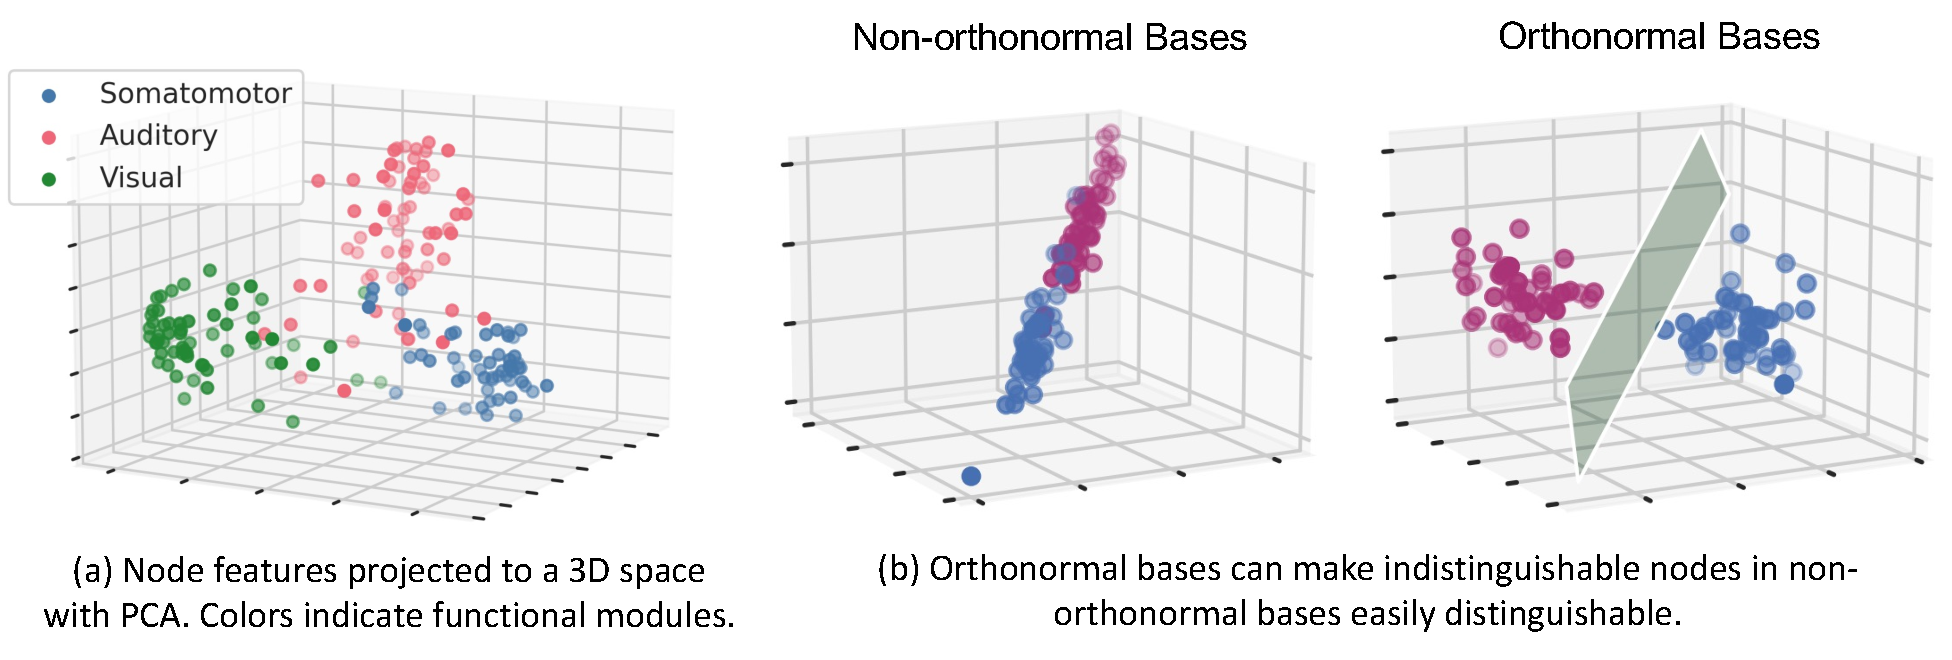
\includegraphics[width=0.8\linewidth]{figures/figure1.pdf}
    \caption{Illustration of the motivations behind \pooling.}
    \label{fig:motivation}
\end{figure*}

In this work, we propose to develop \methodfull (\methodtable), which leverages the unique properties of brain network data to fully unleash the power of Transformer-based models for brain network analysis. Specifically, motivated by previous findings on effective GNN designs for brain networks~\citep{braingb}, we propose to use the effective initial node features of connection profiles. Empirical analysis shows that connection profiles naturally provide positional features for Transformer-based models and avoid the costly computations of eigenvalues or eigenvectors. Moreover, recent work demonstrates that GNNs trained on learnable graph structures can achieve superior effectiveness and explainability~\citep{kan2022fbnetgen}. Inspired by this insight, we propose to learn fully pairwise attention weights with Transformer-based models, which resembles the process of learning predictive brain network structures towards downstream tasks.
 
One step further, when GNNs are used for brain network analysis, a graph-level embedding needs to be generated through a readout function based on the learned node embeddings~\cite{BrainNetCNN, li2020braingnn, braingb}. As is shown in Figure \ref{fig:motivation}(a), a property of brain networks is that brain regions (nodes) belonging to the same functional modules often share similar behaviors regarding activations and deactivations in response to various stimulations~\cite{functionalmodule}. Unfortunately, the current labeling of functional modules is rather empirical and far from accurate. For example,~\cite{akiki2019determining} provides more than 100 different functional module organizations based on hierarchical clustering. In order to leverage the natural functions of brain regions without the limitation of inaccurate functional module labels, we design a new global pooling operator, \pooling, where the graph-level embeddings are pooled from clusters of functionally similar nodes through soft clustering with orthonormal projection.  
Specifically, we first devise a self-supervised mechanism based on~\cite{xie2016unsupervised} to jointly assign soft clusters to brain regions while learning their individual embeddings. To further facilitate the learning of clusters and embeddings, we design an orthonormal projection and theoretically prove its effectiveness in distinguishing embeddings across clusters, thus obtaining expressive graph-level embeddings after the global pooling, as illustrated in Figure \ref{fig:motivation}(b).

Finally, the lack of open-access datasets has been a non-negligible challenge for brain network analysis. The strict access restrictions and complicated extraction/preprocessing of brain networks from fMRI data limit the development of machine learning models for brain network analysis. Specifically, among all the large-scale publicly available fMRI datasets in literature, ABIDE~\citep{abide} is the only one provided with extracted brain networks fully accessible without permission requirements. However, ABIDE is aggregated from 17 international sites with different scanners and acquisition parameters. This inter-site variability conceals inter-group differences that are really meaningful, which is reflected in the unstable training performance and the significant gap between validation and testing performance in practice. To address these limitations, we propose to apply a stratified sampling method in the dataset splitting process and standardize a fair evaluation pipeline for meaningful model comparison on the ABIDE dataset. Our extensive experiments on this public ABIDE dataset and a restricted ABCD dataset~\cite{ABCD} show significant improvements brought by our proposed \methodfull.